% Options for packages loaded elsewhere
\PassOptionsToPackage{unicode}{hyperref}
\PassOptionsToPackage{hyphens}{url}
%
\documentclass[
]{article}
\usepackage{amsmath,amssymb}
\usepackage{iftex}
\ifPDFTeX
  \usepackage[T1]{fontenc}
  \usepackage[utf8]{inputenc}
  \usepackage{textcomp} % provide euro and other symbols
\else % if luatex or xetex
  \usepackage{unicode-math} % this also loads fontspec
  \defaultfontfeatures{Scale=MatchLowercase}
  \defaultfontfeatures[\rmfamily]{Ligatures=TeX,Scale=1}
\fi
\usepackage{lmodern}
\ifPDFTeX\else
  % xetex/luatex font selection
\fi
% Use upquote if available, for straight quotes in verbatim environments
\IfFileExists{upquote.sty}{\usepackage{upquote}}{}
\IfFileExists{microtype.sty}{% use microtype if available
  \usepackage[]{microtype}
  \UseMicrotypeSet[protrusion]{basicmath} % disable protrusion for tt fonts
}{}
\makeatletter
\@ifundefined{KOMAClassName}{% if non-KOMA class
  \IfFileExists{parskip.sty}{%
    \usepackage{parskip}
  }{% else
    \setlength{\parindent}{0pt}
    \setlength{\parskip}{6pt plus 2pt minus 1pt}}
}{% if KOMA class
  \KOMAoptions{parskip=half}}
\makeatother
\usepackage{xcolor}
\usepackage[margin=1in]{geometry}
\usepackage{color}
\usepackage{fancyvrb}
\newcommand{\VerbBar}{|}
\newcommand{\VERB}{\Verb[commandchars=\\\{\}]}
\DefineVerbatimEnvironment{Highlighting}{Verbatim}{commandchars=\\\{\}}
% Add ',fontsize=\small' for more characters per line
\usepackage{framed}
\definecolor{shadecolor}{RGB}{248,248,248}
\newenvironment{Shaded}{\begin{snugshade}}{\end{snugshade}}
\newcommand{\AlertTok}[1]{\textcolor[rgb]{0.94,0.16,0.16}{#1}}
\newcommand{\AnnotationTok}[1]{\textcolor[rgb]{0.56,0.35,0.01}{\textbf{\textit{#1}}}}
\newcommand{\AttributeTok}[1]{\textcolor[rgb]{0.13,0.29,0.53}{#1}}
\newcommand{\BaseNTok}[1]{\textcolor[rgb]{0.00,0.00,0.81}{#1}}
\newcommand{\BuiltInTok}[1]{#1}
\newcommand{\CharTok}[1]{\textcolor[rgb]{0.31,0.60,0.02}{#1}}
\newcommand{\CommentTok}[1]{\textcolor[rgb]{0.56,0.35,0.01}{\textit{#1}}}
\newcommand{\CommentVarTok}[1]{\textcolor[rgb]{0.56,0.35,0.01}{\textbf{\textit{#1}}}}
\newcommand{\ConstantTok}[1]{\textcolor[rgb]{0.56,0.35,0.01}{#1}}
\newcommand{\ControlFlowTok}[1]{\textcolor[rgb]{0.13,0.29,0.53}{\textbf{#1}}}
\newcommand{\DataTypeTok}[1]{\textcolor[rgb]{0.13,0.29,0.53}{#1}}
\newcommand{\DecValTok}[1]{\textcolor[rgb]{0.00,0.00,0.81}{#1}}
\newcommand{\DocumentationTok}[1]{\textcolor[rgb]{0.56,0.35,0.01}{\textbf{\textit{#1}}}}
\newcommand{\ErrorTok}[1]{\textcolor[rgb]{0.64,0.00,0.00}{\textbf{#1}}}
\newcommand{\ExtensionTok}[1]{#1}
\newcommand{\FloatTok}[1]{\textcolor[rgb]{0.00,0.00,0.81}{#1}}
\newcommand{\FunctionTok}[1]{\textcolor[rgb]{0.13,0.29,0.53}{\textbf{#1}}}
\newcommand{\ImportTok}[1]{#1}
\newcommand{\InformationTok}[1]{\textcolor[rgb]{0.56,0.35,0.01}{\textbf{\textit{#1}}}}
\newcommand{\KeywordTok}[1]{\textcolor[rgb]{0.13,0.29,0.53}{\textbf{#1}}}
\newcommand{\NormalTok}[1]{#1}
\newcommand{\OperatorTok}[1]{\textcolor[rgb]{0.81,0.36,0.00}{\textbf{#1}}}
\newcommand{\OtherTok}[1]{\textcolor[rgb]{0.56,0.35,0.01}{#1}}
\newcommand{\PreprocessorTok}[1]{\textcolor[rgb]{0.56,0.35,0.01}{\textit{#1}}}
\newcommand{\RegionMarkerTok}[1]{#1}
\newcommand{\SpecialCharTok}[1]{\textcolor[rgb]{0.81,0.36,0.00}{\textbf{#1}}}
\newcommand{\SpecialStringTok}[1]{\textcolor[rgb]{0.31,0.60,0.02}{#1}}
\newcommand{\StringTok}[1]{\textcolor[rgb]{0.31,0.60,0.02}{#1}}
\newcommand{\VariableTok}[1]{\textcolor[rgb]{0.00,0.00,0.00}{#1}}
\newcommand{\VerbatimStringTok}[1]{\textcolor[rgb]{0.31,0.60,0.02}{#1}}
\newcommand{\WarningTok}[1]{\textcolor[rgb]{0.56,0.35,0.01}{\textbf{\textit{#1}}}}
\usepackage{longtable,booktabs,array}
\usepackage{calc} % for calculating minipage widths
% Correct order of tables after \paragraph or \subparagraph
\usepackage{etoolbox}
\makeatletter
\patchcmd\longtable{\par}{\if@noskipsec\mbox{}\fi\par}{}{}
\makeatother
% Allow footnotes in longtable head/foot
\IfFileExists{footnotehyper.sty}{\usepackage{footnotehyper}}{\usepackage{footnote}}
\makesavenoteenv{longtable}
\usepackage{graphicx}
\makeatletter
\def\maxwidth{\ifdim\Gin@nat@width>\linewidth\linewidth\else\Gin@nat@width\fi}
\def\maxheight{\ifdim\Gin@nat@height>\textheight\textheight\else\Gin@nat@height\fi}
\makeatother
% Scale images if necessary, so that they will not overflow the page
% margins by default, and it is still possible to overwrite the defaults
% using explicit options in \includegraphics[width, height, ...]{}
\setkeys{Gin}{width=\maxwidth,height=\maxheight,keepaspectratio}
% Set default figure placement to htbp
\makeatletter
\def\fps@figure{htbp}
\makeatother
\setlength{\emergencystretch}{3em} % prevent overfull lines
\providecommand{\tightlist}{%
  \setlength{\itemsep}{0pt}\setlength{\parskip}{0pt}}
\setcounter{secnumdepth}{5}
\ifLuaTeX
  \usepackage{selnolig}  % disable illegal ligatures
\fi
\usepackage{bookmark}
\IfFileExists{xurl.sty}{\usepackage{xurl}}{} % add URL line breaks if available
\urlstyle{same}
\hypersetup{
  pdftitle={Analysis of Ontario wages in relation to economic factors based on Ontario Data Catalogue (1997-2019)},
  pdfauthor={Borys Łangowicz (1010725967); Kian Dianati (1010205485)},
  hidelinks,
  pdfcreator={LaTeX via pandoc}}

\title{Analysis of Ontario wages in relation to economic factors based
on Ontario Data Catalogue (1997-2019)}
\author{Borys Łangowicz (1010725967) \and Kian Dianati (1010205485)}
\date{2024-04-05}

\begin{document}
\maketitle

\section{Loading the Data}\label{loading-the-data}

We will use the following data sets:

\begin{Shaded}
\begin{Highlighting}[]
\NormalTok{wages }\OtherTok{=} \FunctionTok{read.csv}\NormalTok{(}\StringTok{"wages.csv"}\NormalTok{) }\SpecialCharTok{\%\textgreater{}\%} \FunctionTok{mutate\_if}\NormalTok{(is.character, str\_trim)}

\CommentTok{\# Clean age ranges}
\CommentTok{\# Want to achieve:}
\CommentTok{\# 15{-}24 DONE}
\CommentTok{\# 25{-}34 DONE}
\CommentTok{\# 35{-}54 // 25{-}54 minus 25{-}34}
\CommentTok{\# 55{-}64 // 25{-}64 minus 25{-}54}
\CommentTok{\# 65+ // 55+ minus 55{-}64}

\CommentTok{\#wages \textless{}{-} wages \%\textgreater{}\% group\_by(YEAR, Geography, Type.of.work, Wages, )}

\NormalTok{wages}\SpecialCharTok{$}\NormalTok{Education.level }\OtherTok{=}
  \FunctionTok{factor}\NormalTok{(wages}\SpecialCharTok{$}\NormalTok{Education.level,}
         \AttributeTok{levels =} \FunctionTok{c}\NormalTok{(}\StringTok{"Above bachelor\textquotesingle{}s degree"}\NormalTok{,}
                    \StringTok{"Bachelor\textquotesingle{}s degree"}\NormalTok{,}
                    \StringTok{"University certificate below bachelors degree"}\NormalTok{,}
                    \StringTok{"University degree"}\NormalTok{,}
                    \StringTok{"Community college, CEGEP"}\NormalTok{,}
                    \StringTok{"Trade certificate or diploma"}\NormalTok{,}
                    \StringTok{"Post{-}secondary certificate or diploma"}\NormalTok{,}
                    \StringTok{"Some post{-}secondary"}\NormalTok{,}
                    \StringTok{"High school graduate"}\NormalTok{,}
                    \StringTok{"Some high school"}\NormalTok{,}
                    \StringTok{"PSE  (5,6,7,8,9))"}\NormalTok{,}
                    \StringTok{"No PSE  (0,1,2,3,4)"}\NormalTok{,}
                    \StringTok{"0 {-} 8  years"}\NormalTok{,}
                    \StringTok{"Total, all education levels"}\NormalTok{),}
         \AttributeTok{ordered =} \ConstantTok{TRUE}\NormalTok{)}

\NormalTok{wages}\SpecialCharTok{$}\NormalTok{Age.group }\OtherTok{=}
  \FunctionTok{factor}\NormalTok{(wages}\SpecialCharTok{$}\NormalTok{Age.group,}
         \AttributeTok{levels =} \FunctionTok{c}\NormalTok{(}\StringTok{"25{-}64 years"}\NormalTok{,}
                    \StringTok{"25{-}54 years"}\NormalTok{,}
                    \StringTok{"25{-}34 years"}\NormalTok{,}
                    \StringTok{"20{-}34 years"}\NormalTok{,}
                    \StringTok{"15{-}24 years"}\NormalTok{,}
                    \StringTok{"55 years and over"}\NormalTok{,}
                    \StringTok{"25 years and over"}\NormalTok{,}
                    \StringTok{"15 years and over"}\NormalTok{),}
         \AttributeTok{ordered =} \ConstantTok{TRUE}\NormalTok{)}

\CommentTok{\# Fuel}
\NormalTok{fuel }\OtherTok{=} \FunctionTok{read.csv}\NormalTok{(}\StringTok{"fuel.csv"}\NormalTok{) }\SpecialCharTok{\%\textgreater{}\%} \FunctionTok{mutate\_if}\NormalTok{(is.character, str\_trim)}

\NormalTok{fuel }\OtherTok{\textless{}{-}}\NormalTok{ fuel }\SpecialCharTok{\%\textgreater{}\%} \FunctionTok{rename}\NormalTok{(}
  \AttributeTok{Toronto.West =}\NormalTok{ Toronto.West.Ouest,}
  \AttributeTok{Toronto.East =}\NormalTok{ Toronto.East.Est,}
  \AttributeTok{St.Catharine =}\NormalTok{ St..Catharine.s,}
  \AttributeTok{Ontario.Average =}\NormalTok{ Ontario.Average.Moyenne.provinciale,}
  \AttributeTok{Southern.Average.Ontario =}\NormalTok{ Southern.Average.Moyenne.du.sud.de.l.Ontario,}
  \AttributeTok{Northern.Average.Ontario =}\NormalTok{ Northern.Average.Moyenne.du.nord.de.l.Ontario }
\NormalTok{) }\SpecialCharTok{\%\textgreater{}\%} \FunctionTok{select}\NormalTok{(}\SpecialCharTok{!}\NormalTok{(Type.de.carburant)) }
\end{Highlighting}
\end{Shaded}

\section{Description of the Data set}\label{description-of-the-data-set}

\subsection{Wages by education level}\label{wages-by-education-level}

The \texttt{wages} data set includes the average weekly wages rates by
education level and immigration status for Canada and Ontario in the
years from 1997 to 2019. It includes the following columns:

\begin{Shaded}
\begin{Highlighting}[]
\FunctionTok{names}\NormalTok{(wages)}
\end{Highlighting}
\end{Shaded}

\begin{verbatim}
## [1] "YEAR"            "Geography"       "Type.of.work"    "Wages"          
## [5] "Education.level" "Age.group"       "Both.Sexes"      "Male"           
## [9] "Female"
\end{verbatim}

\begin{enumerate}
\def\labelenumi{\arabic{enumi}.}
\tightlist
\item
  \texttt{YEAR}: Indicates the year in which the data was collected.
\item
  \texttt{Geography}: Indicates the region from which the data was
  collected. Its possible values include Canada as well as the Canadian
  provinces and territories.
\item
  \texttt{Type.of.work}: Indicates whether the data in the row is for
  full-time employees or part-time employees or both.
\item
  \texttt{Wages}:

  \begin{enumerate}
  \def\labelenumii{\arabic{enumii}.}
  \tightlist
  \item
    \texttt{Total\ employees}: The number of employees in the given age
    range, education level, and job status.
  \item
    \texttt{Average\ hourly\ wage\ rate}: The average hourly wage of the
    employees in the given age range, education level, and job status.
  \item
    And so on for \texttt{Average\ weekly\ wage\ rate},
    \texttt{Median\ hourly\ wage\ rate}, and
    \texttt{Median\ weekly\ wage\ rate}.
  \end{enumerate}
\item
  \texttt{Education.level}: Indicates the level of education. It can
  include the following:
\end{enumerate}

\begin{longtable}[]{@{}l@{}}
\toprule\noalign{}
Education.level \\
\midrule\noalign{}
\endhead
\bottomrule\noalign{}
\endlastfoot
Above bachelor's degree \\
Bachelor's degree \\
University certificate below bachelors degree \\
University degree \\
Community college, CEGEP \\
Trade certificate or diploma \\
Post-secondary certificate or diploma \\
Some post-secondary \\
High school graduate \\
Some high school \\
PSE (5,6,7,8,9)) \\
No PSE (0,1,2,3,4) \\
0 - 8 years \\
Total, all education levels \\
\end{longtable}

\begin{enumerate}
\def\labelenumi{\arabic{enumi}.}
\setcounter{enumi}{5}
\tightlist
\item
  \texttt{Age.group}: Indicates the age range of the individuals under
  consideration. It can include the following:
\end{enumerate}

\begin{longtable}[]{@{}l@{}}
\toprule\noalign{}
Age.group \\
\midrule\noalign{}
\endhead
\bottomrule\noalign{}
\endlastfoot
25-64 years \\
25-54 years \\
25-34 years \\
20-34 years \\
15-24 years \\
55 years and over \\
25 years and over \\
15 years and over \\
\end{longtable}

\begin{enumerate}
\def\labelenumi{\arabic{enumi}.}
\setcounter{enumi}{6}
\tightlist
\item
  \texttt{Both.sexes}: The data not seperated by gender.
\item
  \texttt{Male}: The data for males.
\item
  \texttt{Female}: The data for females.
\end{enumerate}

\subsection{Fuels price survey
information}\label{fuels-price-survey-information}

\begin{Shaded}
\begin{Highlighting}[]
\FunctionTok{names}\NormalTok{(fuel)}
\end{Highlighting}
\end{Shaded}

\begin{verbatim}
##  [1] "Date"                     "Ottawa"                  
##  [3] "Toronto.West"             "Toronto.East"            
##  [5] "Windsor"                  "London"                  
##  [7] "Peterborough"             "St.Catharine"            
##  [9] "Sudbury"                  "Sault.Saint.Marie"       
## [11] "Thunder.Bay"              "North.Bay"               
## [13] "Timmins"                  "Kenora"                  
## [15] "Parry.Sound"              "Ontario.Average"         
## [17] "Southern.Average.Ontario" "Northern.Average.Ontario"
## [19] "Fuel.Type"
\end{verbatim}

TODODODODODOODODODO

\section{The Background of the Data}\label{the-background-of-the-data}

The labor and demographic dataset from the Ministry of Labour,
Immigration, Training, and Skills Development provides insights into
Ontario's workforce demographics, including age groups, employment
types, educational levels, wages, and immigration statuses. It is
annually updated and used by policymakers, researchers, and economists
to inform decisions regarding education, training, workforce
development, and immigration policies in the province.

Additionally, fuel price survey information from the Ministry of Energy
offers weekly retail prices for gasoline, diesel, auto propane, and
compressed natural gas across ten Ontario markets. This data aids in
monitoring fuel price fluctuations and analyzing trends in the energy
sector, supporting research and analysis efforts in economics,
environmental studies, and energy policy.

\section{Overall Research Question}\label{overall-research-question}

\subsection{Trend Analysis}\label{trend-analysis}

\begin{itemize}
\tightlist
\item
  How has the average hourly wage rate changed over the years across
  different age groups?
\item
  Are there any noticeable trends in the median weekly wage rate for
  full-time employees over the past decade?
\item
  What is the overall trend in the number of full-time employees versus
  part-time employees across different age groups?
\end{itemize}

\subsection{Regional Disparities}\label{regional-disparities}

\begin{itemize}
\tightlist
\item
  How do average hourly wage rates vary between different Canadian
  provinces and territories?
\item
  Are there significant differences in the employment rates between
  urban and rural areas within a specific province?
\end{itemize}

\subsection{Educational Attainment}\label{educational-attainment}

\begin{itemize}
\tightlist
\item
  How does the average hourly wage rate differ across various education
  levels?
\item
  Are there any trends in the employment rates based on different levels
  of education attainment?
\item
  Is there a correlation between educational attainment and the
  likelihood of being employed full-time versus part-time?
\end{itemize}

\subsection{Age Groups Analysis}\label{age-groups-analysis}

\begin{itemize}
\tightlist
\item
  How do wage rates vary across different age groups, and is there a
  trend in wage growth as individuals age?
\item
  Are there noticeable differences in employment rates between younger
  and older age groups?
\item
  What is the distribution of educational attainment among different age
  groups, and how does it correlate with employment status and wage
  rates?
\end{itemize}

\subsection{Gender Analysis}\label{gender-analysis}

\begin{itemize}
\tightlist
\item
  Is there a significant gender wage gap, and how has it evolved over
  time?
\item
  Are there differences in the distribution of employment types
  (full-time vs.~part-time) between males and females?
\item
  How does educational attainment affect the gender wage gap within
  specific age groups or regions?
\end{itemize}

\subsection{Overall Employment Trends}\label{overall-employment-trends}

\begin{itemize}
\tightlist
\item
  How has the total number of employees changed over the years?
\item
  Are there seasonal variations in employment rates or wage rates within
  certain industries?
\item
  What industries or sectors have shown the highest growth in employment
  rates, and how does this correlate with wage rates?
\end{itemize}

\section{Summary}\label{summary}

\subsection{How has the average hourly wage rate changed over the years
across different age
groups?}\label{how-has-the-average-hourly-wage-rate-changed-over-the-years-across-different-age-groups}

\begin{Shaded}
\begin{Highlighting}[]
\NormalTok{avg\_wage\_by\_age }\OtherTok{\textless{}{-}}\NormalTok{ wages }\SpecialCharTok{\%\textgreater{}\%}
  \FunctionTok{filter}\NormalTok{(Wages }\SpecialCharTok{==} \StringTok{"Average hourly wage rate"}\NormalTok{,}
\NormalTok{         Geography }\SpecialCharTok{==} \StringTok{"Canada"}\NormalTok{,}
\NormalTok{         Type.of.work }\SpecialCharTok{==} \StringTok{"Full{-}time"}\NormalTok{,}
\NormalTok{         Education.level }\SpecialCharTok{==} \StringTok{"Total, all education levels"}\NormalTok{) }\SpecialCharTok{\%\textgreater{}\%}
  \FunctionTok{select}\NormalTok{(YEAR, Age.group, Both.Sexes) }\SpecialCharTok{\%\textgreater{}\%}
  \FunctionTok{group\_by}\NormalTok{(YEAR, Age.group) }\SpecialCharTok{\%\textgreater{}\%}
  \FunctionTok{summarise}\NormalTok{(}\AttributeTok{Avg\_Hourly\_Wage =} \FunctionTok{mean}\NormalTok{(Both.Sexes))}
\end{Highlighting}
\end{Shaded}

\begin{verbatim}
## `summarise()` has grouped output by 'YEAR'. You can override using the
## `.groups` argument.
\end{verbatim}

\begin{Shaded}
\begin{Highlighting}[]
\FunctionTok{kable}\NormalTok{(avg\_wage\_by\_age }\SpecialCharTok{\%\textgreater{}\%}
  \FunctionTok{pivot\_wider}\NormalTok{(}\AttributeTok{names\_from =}\NormalTok{ Age.group, }\AttributeTok{values\_from =}\NormalTok{ Avg\_Hourly\_Wage))}
\end{Highlighting}
\end{Shaded}

\begin{longtable}[]{@{}
  >{\raggedleft\arraybackslash}p{(\columnwidth - 16\tabcolsep) * \real{0.0420}}
  >{\raggedleft\arraybackslash}p{(\columnwidth - 16\tabcolsep) * \real{0.1008}}
  >{\raggedleft\arraybackslash}p{(\columnwidth - 16\tabcolsep) * \real{0.1008}}
  >{\raggedleft\arraybackslash}p{(\columnwidth - 16\tabcolsep) * \real{0.1008}}
  >{\raggedleft\arraybackslash}p{(\columnwidth - 16\tabcolsep) * \real{0.1008}}
  >{\raggedleft\arraybackslash}p{(\columnwidth - 16\tabcolsep) * \real{0.1008}}
  >{\raggedleft\arraybackslash}p{(\columnwidth - 16\tabcolsep) * \real{0.1513}}
  >{\raggedleft\arraybackslash}p{(\columnwidth - 16\tabcolsep) * \real{0.1513}}
  >{\raggedleft\arraybackslash}p{(\columnwidth - 16\tabcolsep) * \real{0.1513}}@{}}
\toprule\noalign{}
\begin{minipage}[b]{\linewidth}\raggedleft
YEAR
\end{minipage} & \begin{minipage}[b]{\linewidth}\raggedleft
25-64 years
\end{minipage} & \begin{minipage}[b]{\linewidth}\raggedleft
25-54 years
\end{minipage} & \begin{minipage}[b]{\linewidth}\raggedleft
25-34 years
\end{minipage} & \begin{minipage}[b]{\linewidth}\raggedleft
20-34 years
\end{minipage} & \begin{minipage}[b]{\linewidth}\raggedleft
15-24 years
\end{minipage} & \begin{minipage}[b]{\linewidth}\raggedleft
55 years and over
\end{minipage} & \begin{minipage}[b]{\linewidth}\raggedleft
25 years and over
\end{minipage} & \begin{minipage}[b]{\linewidth}\raggedleft
15 years and over
\end{minipage} \\
\midrule\noalign{}
\endhead
\bottomrule\noalign{}
\endlastfoot
1997 & 17.41 & 17.35 & 15.29 & 14.08 & 9.82 & 17.92 & 17.40 & 16.54 \\
1998 & 17.64 & 17.57 & 15.66 & 14.41 & 10.06 & 18.15 & 17.62 & 16.76 \\
1999 & 18.13 & 18.06 & 16.11 & 14.77 & 10.33 & 18.65 & 18.11 & 17.19 \\
2000 & 18.69 & 18.63 & 16.72 & 15.31 & 10.81 & 19.04 & 18.67 & 17.72 \\
2001 & 19.28 & 19.23 & 17.48 & 15.97 & 11.21 & 19.63 & 19.27 & 18.29 \\
2002 & 19.87 & 19.80 & 17.94 & 16.34 & 11.37 & 20.19 & 19.84 & 18.83 \\
2003 & 20.28 & 20.19 & 18.15 & 16.55 & 11.66 & 20.85 & 20.26 & 19.24 \\
2004 & 20.80 & 20.70 & 18.54 & 16.88 & 11.77 & 21.31 & 20.77 & 19.71 \\
2005 & 21.44 & 21.32 & 19.25 & 17.50 & 12.23 & 21.98 & 21.41 & 20.32 \\
2006 & 22.12 & 22.03 & 19.94 & 18.15 & 12.84 & 22.56 & 22.10 & 20.99 \\
2007 & 22.91 & 22.84 & 20.77 & 18.94 & 13.40 & 23.07 & 22.87 & 21.74 \\
2008 & 23.86 & 23.77 & 21.69 & 19.81 & 14.06 & 24.16 & 23.83 & 22.67 \\
2009 & 24.60 & 24.55 & 22.32 & 20.47 & 14.57 & 24.63 & 24.56 & 23.48 \\
2010 & 25.09 & 24.98 & 22.70 & 20.86 & 14.76 & 25.39 & 25.04 & 23.97 \\
2011 & 25.54 & 25.45 & 23.16 & 21.29 & 15.13 & 25.73 & 25.50 & 24.42 \\
2012 & 26.27 & 26.20 & 23.92 & 21.98 & 15.50 & 26.31 & 26.22 & 25.13 \\
2013 & 26.85 & 26.76 & 24.35 & 22.36 & 15.86 & 27.02 & 26.81 & 25.70 \\
2014 & 27.33 & 27.29 & 24.89 & 22.87 & 16.20 & 27.25 & 27.28 & 26.17 \\
2015 & 28.10 & 28.14 & 25.64 & 23.52 & 16.53 & 27.57 & 28.03 & 26.88 \\
2016 & 28.69 & 28.66 & 26.18 & 24.05 & 16.81 & 28.48 & 28.62 & 27.47 \\
2017 & 29.12 & 29.16 & 26.55 & 24.41 & 17.01 & 28.49 & 29.03 & 27.88 \\
2018 & 29.75 & 29.75 & 27.10 & 25.07 & 17.96 & 29.38 & 29.68 & 28.56 \\
2019 & 30.69 & 30.75 & 27.79 & 25.97 & 19.32 & 30.12 & 30.62 & 29.56 \\
\end{longtable}

\begin{Shaded}
\begin{Highlighting}[]
\FunctionTok{ggplot}\NormalTok{(avg\_wage\_by\_age }\SpecialCharTok{\%\textgreater{}\%} \FunctionTok{filter}\NormalTok{(YEAR }\SpecialCharTok{==} \StringTok{"2019"}\NormalTok{),}
       \FunctionTok{aes}\NormalTok{(}\AttributeTok{x =}\NormalTok{ Age.group, Avg\_Hourly\_Wage)) }\SpecialCharTok{+}
  \FunctionTok{geom\_bar}\NormalTok{(}\AttributeTok{stat =} \StringTok{"identity"}\NormalTok{) }\SpecialCharTok{+}
  \FunctionTok{labs}\NormalTok{(}\AttributeTok{x =} \StringTok{"Age group"}\NormalTok{,}
       \AttributeTok{y =} \StringTok{"Average Hourly Wage"}\NormalTok{,}
       \AttributeTok{title =} \StringTok{"Wage by Age Group in 2019"}\NormalTok{) }\SpecialCharTok{+}
  \FunctionTok{theme}\NormalTok{(}\AttributeTok{text =} \FunctionTok{element\_text}\NormalTok{(}\AttributeTok{size =} \DecValTok{8}\NormalTok{))}
\end{Highlighting}
\end{Shaded}

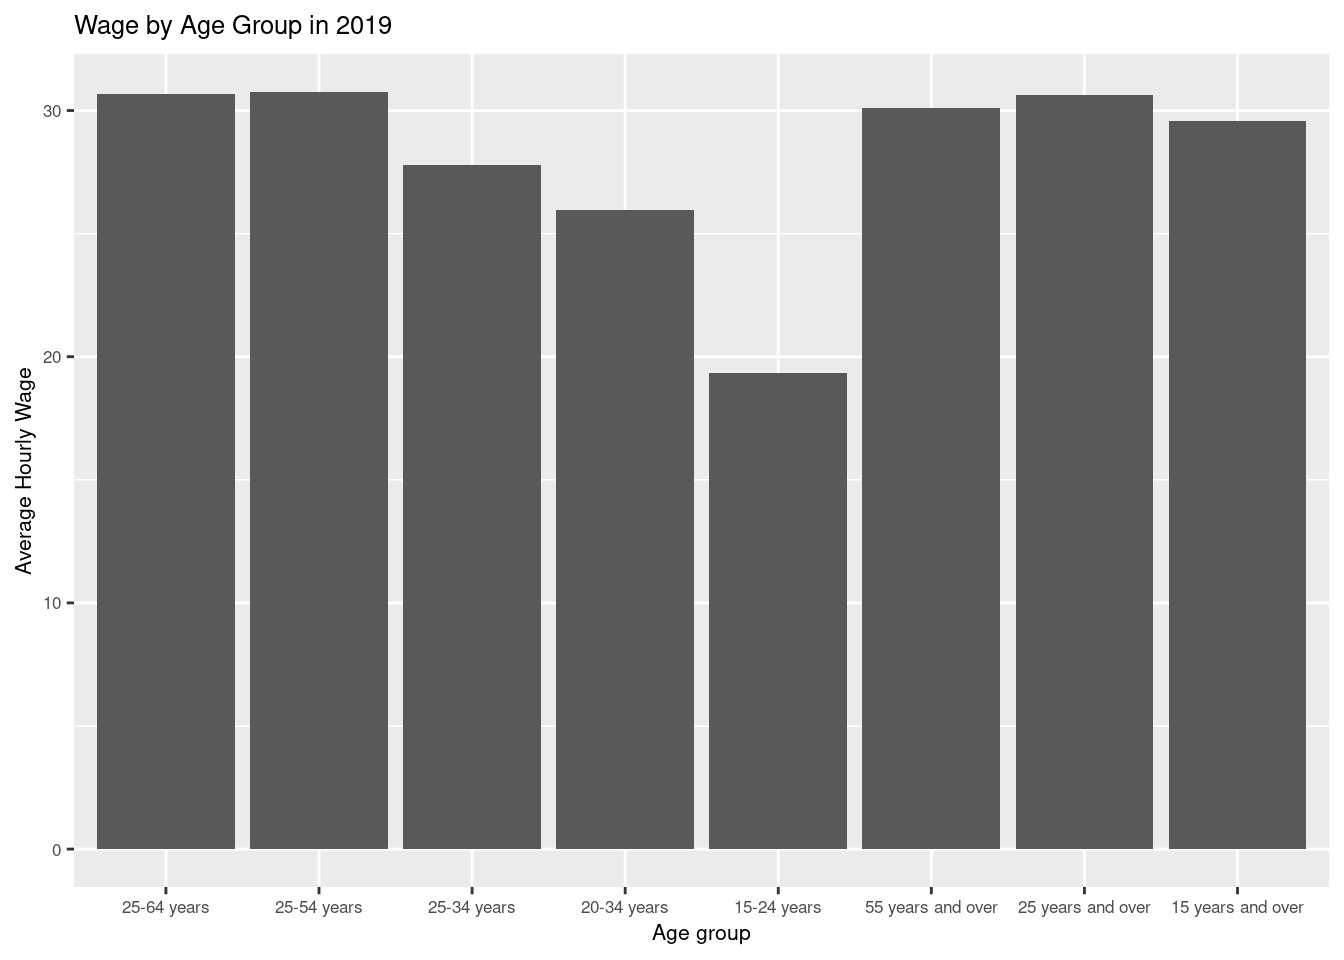
\includegraphics{Wages-Ontario_files/figure-latex/unnamed-chunk-8-1.pdf}

\textbf{From the data, we can observe the following trends:}

\begin{enumerate}
\def\labelenumi{\arabic{enumi}.}
\tightlist
\item
  Across all age groups, there is a general trend of increasing average
  hourly wage rates over the years.
\item
  The wage rates tend to increase with age, with the highest rates
  typically observed in the 55 years and over age group.
\item
  The 15-24 years age group consistently has the lowest average hourly
  wage rates, which gradually increase as individuals move into older
  age groups.
\item
  There is a noticeable increase in wage rates during the late 1990s and
  early 2000s, followed by a slight dip during the economic downturn of
  2008-2009, after which wages steadily increased again.
\end{enumerate}

These observations provide an overview of how the average hourly wage
rates have changed over the years across different age groups.

\subsection{How does the average hourly wage rate differ across various
education levels for different
genders?}\label{how-does-the-average-hourly-wage-rate-differ-across-various-education-levels-for-different-genders}

\begin{Shaded}
\begin{Highlighting}[]
\NormalTok{avg\_wage\_by\_education }\OtherTok{\textless{}{-}}\NormalTok{ wages }\SpecialCharTok{\%\textgreater{}\%}
  \FunctionTok{filter}\NormalTok{(Wages }\SpecialCharTok{==} \StringTok{"Average hourly wage rate"}\NormalTok{, }
\NormalTok{         Geography }\SpecialCharTok{==} \StringTok{"Canada"}\NormalTok{,}
\NormalTok{         Age.group }\SpecialCharTok{==} \StringTok{"15 years and over"}\NormalTok{,}
\NormalTok{         Type.of.work }\SpecialCharTok{==} \StringTok{"Both full{-} and part{-}time"}\NormalTok{) }\SpecialCharTok{\%\textgreater{}\%}
  \FunctionTok{select}\NormalTok{(Education.level, Male, Female) }\SpecialCharTok{\%\textgreater{}\%}
  \FunctionTok{group\_by}\NormalTok{(Education.level) }\SpecialCharTok{\%\textgreater{}\%}
  \FunctionTok{summarise}\NormalTok{(}\AttributeTok{male\_avg =} \FunctionTok{mean}\NormalTok{(Male),}
            \AttributeTok{female\_avg =} \FunctionTok{mean}\NormalTok{(Female))}

\FunctionTok{kable}\NormalTok{(avg\_wage\_by\_education)}
\end{Highlighting}
\end{Shaded}

\begin{longtable}[]{@{}lrr@{}}
\toprule\noalign{}
Education.level & male\_avg & female\_avg \\
\midrule\noalign{}
\endhead
\bottomrule\noalign{}
\endlastfoot
Above bachelor's degree & 33.18565 & 29.29043 \\
Bachelor's degree & 28.89087 & 24.83000 \\
University certificate below bachelors degree & 25.33957 & 21.80435 \\
University degree & 30.29478 & 26.04565 \\
Community college, CEGEP & 23.81000 & 19.74957 \\
Trade certificate or diploma & 23.44783 & 17.01913 \\
Post-secondary certificate or diploma & 23.75652 & 19.35348 \\
Some post-secondary & 18.32478 & 15.12348 \\
High school graduate & 19.64739 & 15.93130 \\
Some high school & 16.34565 & 12.35565 \\
PSE (5,6,7,8,9)) & 26.32174 & 22.16043 \\
No PSE (0,1,2,3,4) & 18.38304 & 14.83043 \\
0 - 8 years & 17.05087 & 12.62870 \\
Total, all education levels & 22.94130 & 19.38304 \\
\end{longtable}

\begin{Shaded}
\begin{Highlighting}[]
\FunctionTok{ggplot}\NormalTok{(avg\_wage\_by\_education }\SpecialCharTok{\%\textgreater{}\%} \FunctionTok{melt}\NormalTok{(),}
       \FunctionTok{aes}\NormalTok{(}\AttributeTok{x =}\NormalTok{ Education.level, }\AttributeTok{fill =}\NormalTok{ variable)) }\SpecialCharTok{+}
  \FunctionTok{geom\_bar}\NormalTok{(}\FunctionTok{aes}\NormalTok{(}\AttributeTok{y =}\NormalTok{ value), }
           \AttributeTok{stat =} \StringTok{"identity"}\NormalTok{, }
           \AttributeTok{alpha =} \FloatTok{0.8}\NormalTok{,}
           \AttributeTok{show.legend =} \ConstantTok{TRUE}\NormalTok{,}
           \AttributeTok{position =} \FunctionTok{position\_identity}\NormalTok{()) }\SpecialCharTok{+}
  \FunctionTok{labs}\NormalTok{(}\AttributeTok{title =} \StringTok{"Average Hourly Wage Rate by Education Level and Gender"}\NormalTok{,}
       \AttributeTok{x =} \StringTok{"Education Level"}\NormalTok{,}
       \AttributeTok{y =} \StringTok{"Average Hourly Wage Rate"}\NormalTok{,}
       \AttributeTok{fill =} \StringTok{"Gender"}\NormalTok{) }\SpecialCharTok{+}
  \FunctionTok{theme}\NormalTok{(}\AttributeTok{axis.text.x =} \FunctionTok{element\_text}\NormalTok{(}\AttributeTok{angle =} \DecValTok{45}\NormalTok{, }\AttributeTok{hjust =} \DecValTok{1}\NormalTok{),}
        \AttributeTok{text =} \FunctionTok{element\_text}\NormalTok{(}\AttributeTok{size =} \DecValTok{8}\NormalTok{),}
        \AttributeTok{legend.position =} \StringTok{"bottom"}\NormalTok{) }\SpecialCharTok{+}
  \FunctionTok{coord\_flip}\NormalTok{()}
\end{Highlighting}
\end{Shaded}

\begin{verbatim}
## Using Education.level as id variables
\end{verbatim}

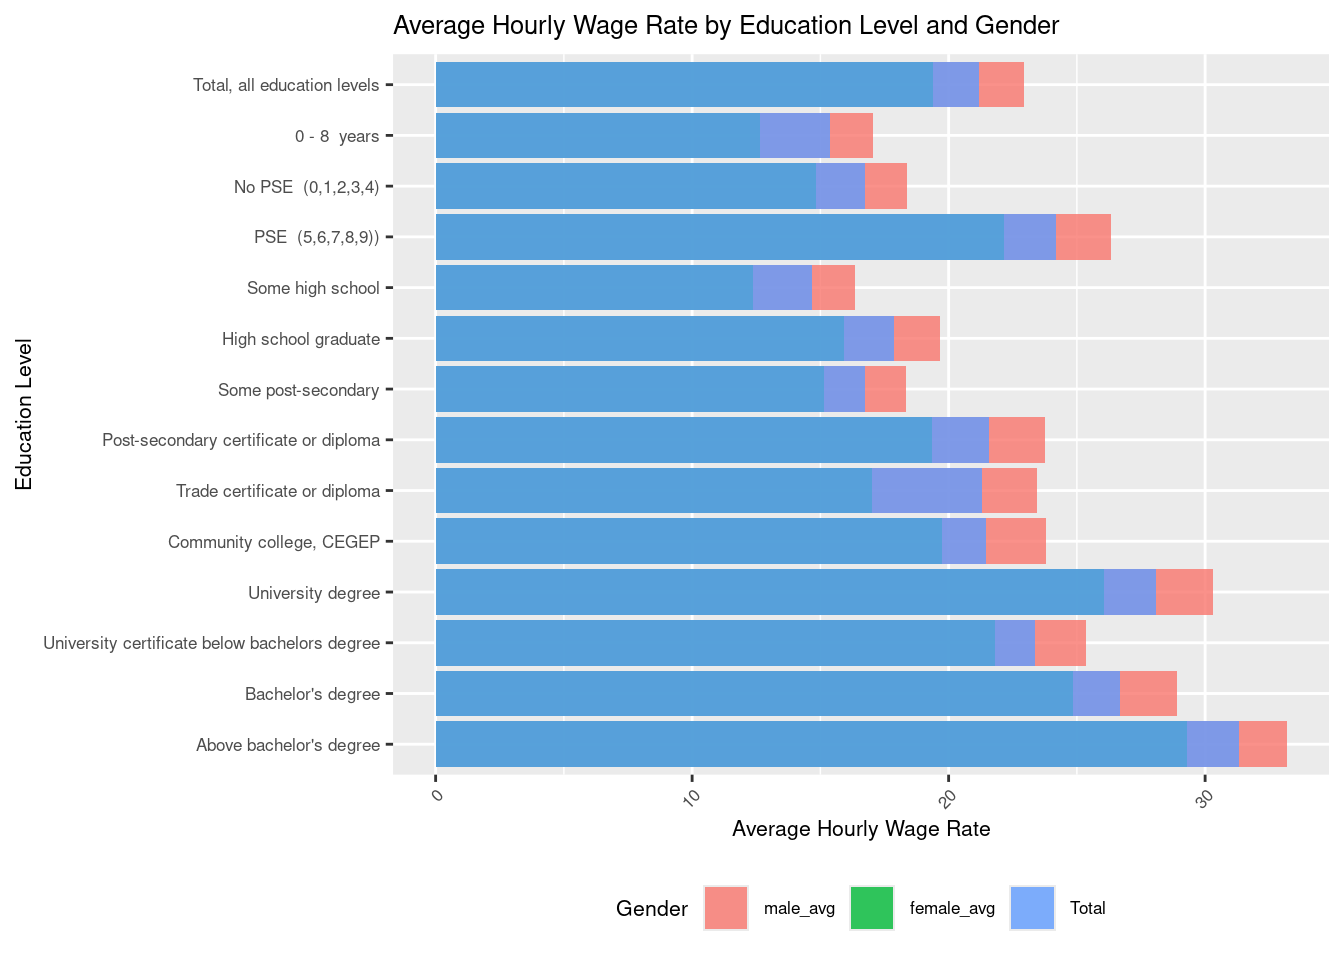
\includegraphics{Wages-Ontario_files/figure-latex/unnamed-chunk-10-1.pdf}

\begin{Shaded}
\begin{Highlighting}[]
\FunctionTok{kable}\NormalTok{(avg\_wage\_by\_education }\SpecialCharTok{\%\textgreater{}\%}
  \FunctionTok{mutate}\NormalTok{(}\AttributeTok{pay.gap =}\NormalTok{ male\_avg }\SpecialCharTok{{-}}\NormalTok{ female\_avg))}
\end{Highlighting}
\end{Shaded}

\begin{longtable}[]{@{}
  >{\raggedright\arraybackslash}p{(\columnwidth - 6\tabcolsep) * \real{0.6133}}
  >{\raggedleft\arraybackslash}p{(\columnwidth - 6\tabcolsep) * \real{0.1200}}
  >{\raggedleft\arraybackslash}p{(\columnwidth - 6\tabcolsep) * \real{0.1467}}
  >{\raggedleft\arraybackslash}p{(\columnwidth - 6\tabcolsep) * \real{0.1200}}@{}}
\toprule\noalign{}
\begin{minipage}[b]{\linewidth}\raggedright
Education.level
\end{minipage} & \begin{minipage}[b]{\linewidth}\raggedleft
male\_avg
\end{minipage} & \begin{minipage}[b]{\linewidth}\raggedleft
female\_avg
\end{minipage} & \begin{minipage}[b]{\linewidth}\raggedleft
pay.gap
\end{minipage} \\
\midrule\noalign{}
\endhead
\bottomrule\noalign{}
\endlastfoot
Above bachelor's degree & 33.18565 & 29.29043 & 3.895217 \\
Bachelor's degree & 28.89087 & 24.83000 & 4.060870 \\
University certificate below bachelors degree & 25.33957 & 21.80435 &
3.535217 \\
University degree & 30.29478 & 26.04565 & 4.249130 \\
Community college, CEGEP & 23.81000 & 19.74957 & 4.060435 \\
Trade certificate or diploma & 23.44783 & 17.01913 & 6.428696 \\
Post-secondary certificate or diploma & 23.75652 & 19.35348 &
4.403043 \\
Some post-secondary & 18.32478 & 15.12348 & 3.201304 \\
High school graduate & 19.64739 & 15.93130 & 3.716087 \\
Some high school & 16.34565 & 12.35565 & 3.990000 \\
PSE (5,6,7,8,9)) & 26.32174 & 22.16043 & 4.161304 \\
No PSE (0,1,2,3,4) & 18.38304 & 14.83043 & 3.552609 \\
0 - 8 years & 17.05087 & 12.62870 & 4.422174 \\
Total, all education levels & 22.94130 & 19.38304 & 3.558261 \\
\end{longtable}

\begin{Shaded}
\begin{Highlighting}[]
\FunctionTok{ggplot}\NormalTok{(avg\_wage\_by\_education }\SpecialCharTok{\%\textgreater{}\%} \FunctionTok{mutate}\NormalTok{(}\AttributeTok{pay.gap =}\NormalTok{ male\_avg }\SpecialCharTok{{-}}\NormalTok{ female\_avg), }
       \FunctionTok{aes}\NormalTok{(}\AttributeTok{x =}\NormalTok{ Education.level, }\AttributeTok{y =}\NormalTok{ pay.gap)) }\SpecialCharTok{+}
  \FunctionTok{geom\_bar}\NormalTok{(}\AttributeTok{stat =} \StringTok{"identity"}\NormalTok{) }\SpecialCharTok{+}
  \FunctionTok{labs}\NormalTok{(}\AttributeTok{y =} \StringTok{"Gender Pay Gap"}\NormalTok{,}
       \AttributeTok{x =} \StringTok{"Education Level"}\NormalTok{,}
       \AttributeTok{title =} \StringTok{"Gender Pay Gap by Education"}\NormalTok{) }\SpecialCharTok{+}
  \FunctionTok{coord\_flip}\NormalTok{()}
\end{Highlighting}
\end{Shaded}

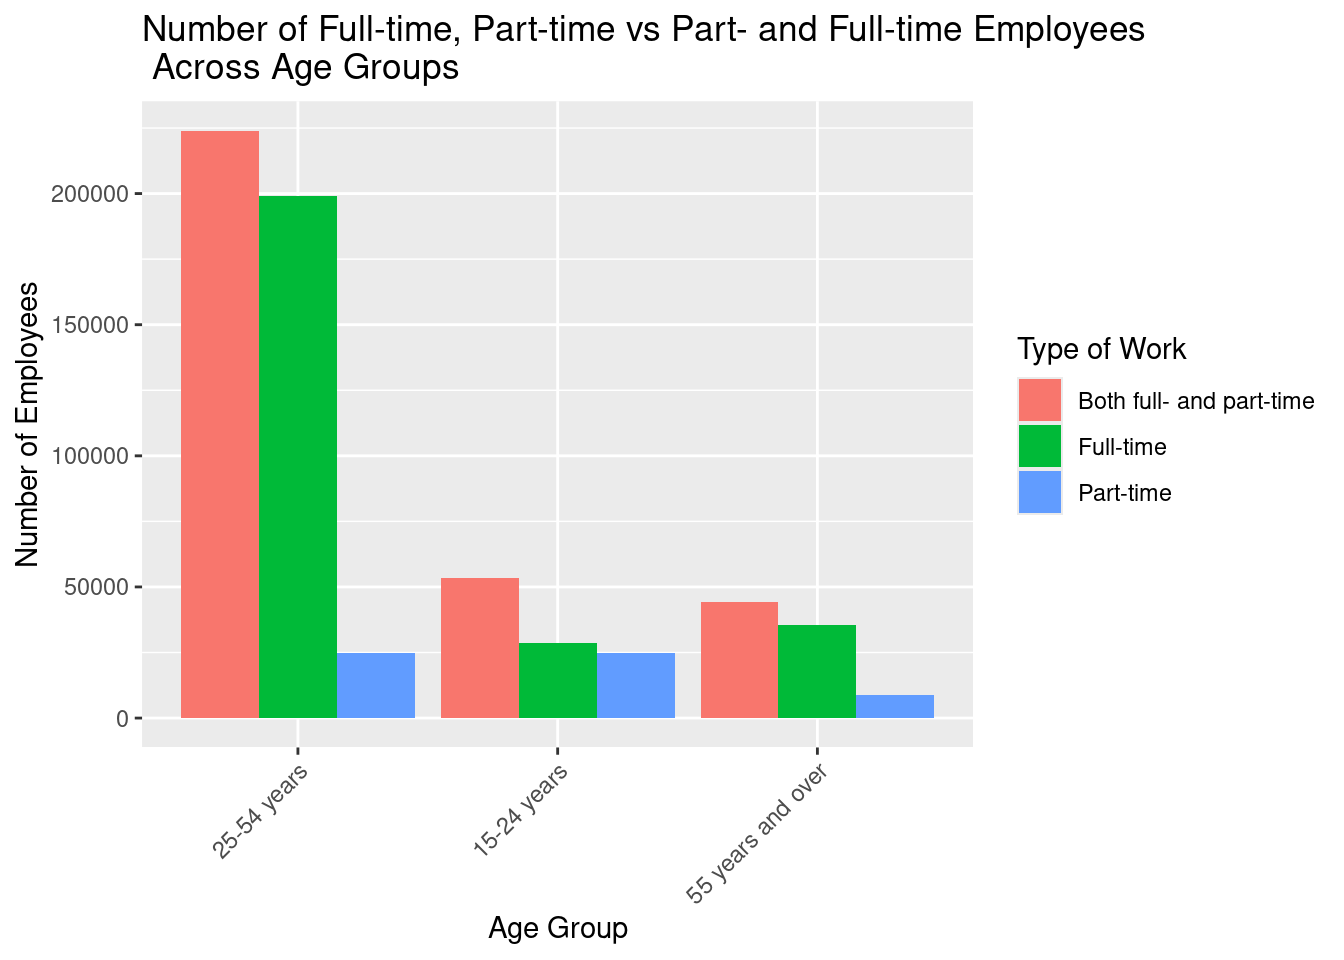
\includegraphics{Wages-Ontario_files/figure-latex/unnamed-chunk-12-1.pdf}

\textbf{Observations:}

\begin{enumerate}
\def\labelenumi{\arabic{enumi}.}
\tightlist
\item
  In almost all cases, the average hourly wage for males is higher than
  for females across various education levels.
\item
  The largest wage gaps are observed at ``Trade certificate or diploma''
  where
\item
  At higher education levels, such as ``Above bachelor's degree'' and
  ``Bachelor's degree'', the wage gap is relatively smaller compared to
  lower education levels but still exists.
\end{enumerate}

These observations highlight disparities in wages between genders across
different education levels, indicating the presence of gender-based wage
inequality.

\subsection{What is the overall trend in the number of full-time
employees versus part-time employees across different age
groups?}\label{what-is-the-overall-trend-in-the-number-of-full-time-employees-versus-part-time-employees-across-different-age-groups}

\begin{Shaded}
\begin{Highlighting}[]
\FunctionTok{unique}\NormalTok{(wages}\SpecialCharTok{$}\NormalTok{Type.of.work)}
\end{Highlighting}
\end{Shaded}

\begin{verbatim}
## [1] "Both full- and part-time" "Full-time"               
## [3] "Part-time"
\end{verbatim}

\begin{Shaded}
\begin{Highlighting}[]
\NormalTok{full\_time\_part\_time }\OtherTok{\textless{}{-}}\NormalTok{ wages }\SpecialCharTok{\%\textgreater{}\%} 
  \FunctionTok{filter}\NormalTok{(Age.group }\SpecialCharTok{\%in\%} \FunctionTok{c}\NormalTok{(}\StringTok{"15{-}24 years"}\NormalTok{, }
                          \StringTok{"25{-}54 years"}\NormalTok{, }
                          \StringTok{"55 years and over"}\NormalTok{)) }\SpecialCharTok{\%\textgreater{}\%}
  \FunctionTok{group\_by}\NormalTok{(Age.group, Type.of.work) }\SpecialCharTok{\%\textgreater{}\%}
  \FunctionTok{summarise}\NormalTok{(}\AttributeTok{Employees =} \FunctionTok{sum}\NormalTok{(Both.Sexes))}
\end{Highlighting}
\end{Shaded}

\begin{verbatim}
## `summarise()` has grouped output by 'Age.group'. You can override using the
## `.groups` argument.
\end{verbatim}

\begin{Shaded}
\begin{Highlighting}[]
\FunctionTok{options}\NormalTok{(}\AttributeTok{scipen =} \DecValTok{999}\NormalTok{)}
\FunctionTok{ggplot}\NormalTok{(full\_time\_part\_time, }
       \FunctionTok{aes}\NormalTok{(}\AttributeTok{x =}\NormalTok{ Age.group, }\AttributeTok{y =}\NormalTok{ Employees, }\AttributeTok{fill =}\NormalTok{ Type.of.work)) }\SpecialCharTok{+}
  \FunctionTok{geom\_bar}\NormalTok{(}\AttributeTok{stat =} \StringTok{"identity"}\NormalTok{, }\AttributeTok{position =} \StringTok{"dodge"}\NormalTok{) }\SpecialCharTok{+}
  \FunctionTok{labs}\NormalTok{(}\AttributeTok{title =} \StringTok{"Number of Full{-}time, Part{-}time vs Part{-} and Full{-}time Employees}\SpecialCharTok{\textbackslash{}n}\StringTok{ Across Age Groups"}\NormalTok{,}
       \AttributeTok{x =} \StringTok{"Age Group"}\NormalTok{,}
       \AttributeTok{y =} \StringTok{"Number of Employees"}\NormalTok{,}
       \AttributeTok{fill =} \StringTok{"Type of Work"}\NormalTok{) }\SpecialCharTok{+}
  \FunctionTok{theme}\NormalTok{(}\AttributeTok{axis.text.x =} \FunctionTok{element\_text}\NormalTok{(}\AttributeTok{angle =} \DecValTok{45}\NormalTok{, }\AttributeTok{hjust =} \DecValTok{1}\NormalTok{))}
\end{Highlighting}
\end{Shaded}

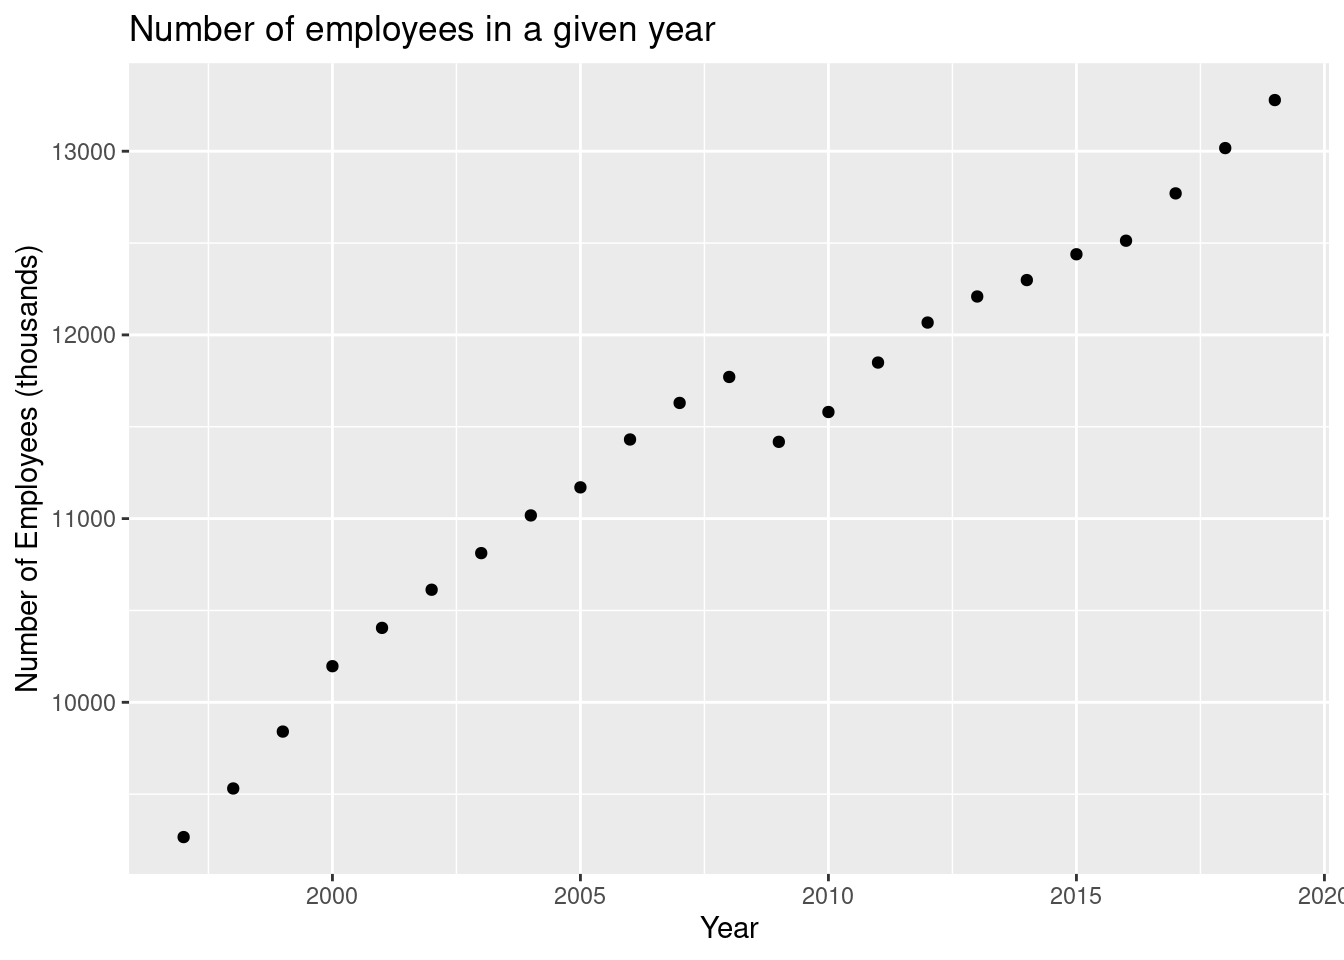
\includegraphics{Wages-Ontario_files/figure-latex/unnamed-chunk-13-1.pdf}

\subsection{What is the relationship between Wages and Fuel
Price?}\label{what-is-the-relationship-between-wages-and-fuel-price}

\begin{Shaded}
\begin{Highlighting}[]
\NormalTok{fuel.year }\OtherTok{=}\NormalTok{ fuel }\SpecialCharTok{\%\textgreater{}\%}
  \FunctionTok{mutate}\NormalTok{(}\AttributeTok{Year =} \FunctionTok{year}\NormalTok{(}\FunctionTok{as.Date}\NormalTok{(Date))) }\SpecialCharTok{\%\textgreater{}\%}
  \FunctionTok{group\_by}\NormalTok{(Year) }\SpecialCharTok{\%\textgreater{}\%}
  \FunctionTok{summarise}\NormalTok{(}\AttributeTok{Avg.Price =} \FunctionTok{mean}\NormalTok{(Ontario.Average))}

\NormalTok{wages.year }\OtherTok{=}\NormalTok{ wages }\SpecialCharTok{\%\textgreater{}\%}
  \FunctionTok{filter}\NormalTok{(Geography }\SpecialCharTok{==} \StringTok{\textquotesingle{}Ontario\textquotesingle{}}\NormalTok{,}
\NormalTok{         Wages }\SpecialCharTok{==} \StringTok{\textquotesingle{}Average hourly wage rate\textquotesingle{}}\NormalTok{,}
\NormalTok{         Type.of.work }\SpecialCharTok{==} \StringTok{\textquotesingle{}Both full{-} and part{-}time\textquotesingle{}}\NormalTok{,}
\NormalTok{         Education.level }\SpecialCharTok{==} \StringTok{\textquotesingle{}Total, all education levels\textquotesingle{}}\NormalTok{,}
\NormalTok{         Age.group }\SpecialCharTok{==} \StringTok{\textquotesingle{}15 years and over\textquotesingle{}}\NormalTok{) }\SpecialCharTok{\%\textgreater{}\%}
  \FunctionTok{select}\NormalTok{(YEAR, Both.Sexes)}

\NormalTok{merged\_data }\OtherTok{\textless{}{-}} \FunctionTok{merge}\NormalTok{(wages.year, fuel.year, }\AttributeTok{by.x =} \StringTok{"YEAR"}\NormalTok{, }\AttributeTok{by.y =} \StringTok{"Year"}\NormalTok{)}

\FunctionTok{ggplot}\NormalTok{(merged\_data, }\FunctionTok{aes}\NormalTok{(}\AttributeTok{x =}\NormalTok{ Both.Sexes, }\AttributeTok{y =}\NormalTok{ Avg.Price)) }\SpecialCharTok{+}
  \FunctionTok{geom\_point}\NormalTok{() }\SpecialCharTok{+}
  \FunctionTok{geom\_smooth}\NormalTok{(}\AttributeTok{method =} \StringTok{"lm"}\NormalTok{) }\SpecialCharTok{+}
  \FunctionTok{labs}\NormalTok{(}\AttributeTok{x =} \StringTok{"Average wage"}\NormalTok{, }
       \AttributeTok{y =} \StringTok{"Average fuel price"}\NormalTok{, }
       \AttributeTok{title =} \StringTok{"Relationship between Wages and Fuel Price"}\NormalTok{)}
\end{Highlighting}
\end{Shaded}

\begin{verbatim}
## `geom_smooth()` using formula = 'y ~ x'
\end{verbatim}

\includegraphics{Wages-Ontario_files/figure-latex/unnamed-chunk-14-1.pdf}

\begin{Shaded}
\begin{Highlighting}[]
\CommentTok{\# fuel and wage vs year}
\FunctionTok{ggplot}\NormalTok{(merged\_data, }\FunctionTok{aes}\NormalTok{(}\AttributeTok{x =}\NormalTok{ YEAR)) }\SpecialCharTok{+}
  \FunctionTok{geom\_line}\NormalTok{(}\FunctionTok{aes}\NormalTok{(}\AttributeTok{y =}\NormalTok{ Both.Sexes, }\AttributeTok{color =} \StringTok{"Both Sexes"}\NormalTok{), }\AttributeTok{size =} \FloatTok{1.5}\NormalTok{) }\SpecialCharTok{+}
  \FunctionTok{geom\_line}\NormalTok{(}\FunctionTok{aes}\NormalTok{(}\AttributeTok{y =}\NormalTok{ Avg.Price, }\AttributeTok{color =} \StringTok{"Avg. Price"}\NormalTok{)) }\SpecialCharTok{+}
  \CommentTok{\# scale\_y\_continuous(sec.axis = sec\_axis(\textasciitilde{}./0.1, name = "Avg. Price")) +}
  \FunctionTok{labs}\NormalTok{(}\AttributeTok{x =} \StringTok{"Year"}\NormalTok{, }\AttributeTok{y =} \StringTok{"Both Sexes"}\NormalTok{, }\AttributeTok{color =} \StringTok{"Legend"}\NormalTok{)}
\end{Highlighting}
\end{Shaded}

\begin{verbatim}
## Warning: Using `size` aesthetic for lines was deprecated in ggplot2 3.4.0.
## i Please use `linewidth` instead.
## This warning is displayed once every 8 hours.
## Call `lifecycle::last_lifecycle_warnings()` to see where this warning was
## generated.
\end{verbatim}

\includegraphics{Wages-Ontario_files/figure-latex/unnamed-chunk-14-2.pdf}

\begin{Shaded}
\begin{Highlighting}[]
\FunctionTok{kable}\NormalTok{(avg\_wage\_by\_education }\SpecialCharTok{\%\textgreater{}\%}
  \FunctionTok{mutate}\NormalTok{(}\AttributeTok{pay.gap =}\NormalTok{ male\_avg }\SpecialCharTok{{-}}\NormalTok{ female\_avg))}
\end{Highlighting}
\end{Shaded}

\begin{longtable}[]{@{}
  >{\raggedright\arraybackslash}p{(\columnwidth - 6\tabcolsep) * \real{0.6133}}
  >{\raggedleft\arraybackslash}p{(\columnwidth - 6\tabcolsep) * \real{0.1200}}
  >{\raggedleft\arraybackslash}p{(\columnwidth - 6\tabcolsep) * \real{0.1467}}
  >{\raggedleft\arraybackslash}p{(\columnwidth - 6\tabcolsep) * \real{0.1200}}@{}}
\toprule\noalign{}
\begin{minipage}[b]{\linewidth}\raggedright
Education.level
\end{minipage} & \begin{minipage}[b]{\linewidth}\raggedleft
male\_avg
\end{minipage} & \begin{minipage}[b]{\linewidth}\raggedleft
female\_avg
\end{minipage} & \begin{minipage}[b]{\linewidth}\raggedleft
pay.gap
\end{minipage} \\
\midrule\noalign{}
\endhead
\bottomrule\noalign{}
\endlastfoot
Above bachelor's degree & 33.18565 & 29.29043 & 3.895217 \\
Bachelor's degree & 28.89087 & 24.83000 & 4.060870 \\
University certificate below bachelors degree & 25.33957 & 21.80435 &
3.535217 \\
University degree & 30.29478 & 26.04565 & 4.249130 \\
Community college, CEGEP & 23.81000 & 19.74957 & 4.060435 \\
Trade certificate or diploma & 23.44783 & 17.01913 & 6.428696 \\
Post-secondary certificate or diploma & 23.75652 & 19.35348 &
4.403043 \\
Some post-secondary & 18.32478 & 15.12348 & 3.201304 \\
High school graduate & 19.64739 & 15.93130 & 3.716087 \\
Some high school & 16.34565 & 12.35565 & 3.990000 \\
PSE (5,6,7,8,9)) & 26.32174 & 22.16043 & 4.161304 \\
No PSE (0,1,2,3,4) & 18.38304 & 14.83043 & 3.552609 \\
0 - 8 years & 17.05087 & 12.62870 & 4.422174 \\
Total, all education levels & 22.94130 & 19.38304 & 3.558261 \\
\end{longtable}

\section{Hypothesis Testing}\label{hypothesis-testing}

\textbf{Null Hypothesis (H0)}: There is no statistically significant
distinction in the average wages between male and female workers
(μ\_male = μ\_female).

\textbf{Alternative Hypothesis (H1)}: There exists a statistically
significant disparity in average wages between male and female workers
(μ\_male ≠ μ\_female). To examine this hypothesis, we can employ a
two-sample t-test to compare the wage distributions of male and female
workers. This entails segregating the dataset into two distinct groups
based on gender: male and female.

The resultant p-value derived from the selected statistical test
indicates the probability of observing a wage difference as extreme as,
or more extreme than, the observed difference, assuming the null
hypothesis holds. If the obtained p-value falls below the predetermined
significance level (typically 0.05), we reject the null hypothesis,
indicating a significant discrepancy in wages between male and female
workers.

Moreover, by computing a confidence interval for the disparity in mean
wages, we can gauge the plausible range of values for the actual
difference between male and female wages.

\begin{Shaded}
\begin{Highlighting}[]
\NormalTok{male\_wages }\OtherTok{\textless{}{-}}\NormalTok{ wages }\SpecialCharTok{\%\textgreater{}\%} \FunctionTok{filter}\NormalTok{(Wages }\SpecialCharTok{==} \StringTok{"Average weekly wage rate"}\NormalTok{) }\SpecialCharTok{\%\textgreater{}\%} \FunctionTok{select}\NormalTok{(Male)}
\NormalTok{female\_wages }\OtherTok{\textless{}{-}}\NormalTok{ wages }\SpecialCharTok{\%\textgreater{}\%} \FunctionTok{filter}\NormalTok{(Wages }\SpecialCharTok{==} \StringTok{"Average weekly wage rate"}\NormalTok{) }\SpecialCharTok{\%\textgreater{}\%} \FunctionTok{select}\NormalTok{(Female)}

\FunctionTok{t.test}\NormalTok{(male\_wages, female\_wages)}
\end{Highlighting}
\end{Shaded}

\begin{verbatim}
## 
##  Welch Two Sample t-test
## 
## data:  male_wages and female_wages
## t = 69.11, df = 155915, p-value < 0.00000000000000022
## alternative hypothesis: true difference in means is not equal to 0
## 95 percent confidence interval:
##  116.8124 123.6314
## sample estimates:
## mean of x mean of y 
##  627.8701  507.6481
\end{verbatim}

\textbf{Conclusions} The outcomes derived from the Welch Two Sample
t-test underscore a significant contrast in average earnings between
male and female workers. With an extraordinarily minute p-value
(\textless{} 0.00000000000000022), there's compelling evidence to
dismiss the null hypothesis, indicating that the mean wages for men and
women diverge significantly. The 95\% confidence interval for the mean
wage discrepancy extends from 116.8124 to 123.6314, suggesting that the
actual difference in wages between male and female workers likely lies
within this interval.

In summary, the findings overwhelmingly advocate for rejecting the null
hypothesis, underscoring a noteworthy disparity in wages between male
and female employees. Specifically, the average wage for male workers
(627.8701) markedly exceeds that of female workers (507.6481).

\section{Bootstrapping}\label{bootstrapping}

\begin{Shaded}
\begin{Highlighting}[]
\FunctionTok{library}\NormalTok{(boot)}

\NormalTok{mean\_fuel\_price }\OtherTok{\textless{}{-}} \ControlFlowTok{function}\NormalTok{(data) \{}
  \FunctionTok{mean}\NormalTok{(data[[}\StringTok{"Toronto.West"}\NormalTok{]])}
\NormalTok{\}}

\FunctionTok{set.seed}\NormalTok{(}\DecValTok{123}\NormalTok{)}
\NormalTok{n\_boot }\OtherTok{\textless{}{-}} \DecValTok{1000} 
\NormalTok{bootstrap\_means }\OtherTok{\textless{}{-}} \FunctionTok{replicate}\NormalTok{(n\_boot, \{}
\NormalTok{  sample\_data }\OtherTok{\textless{}{-}}\NormalTok{ fuel[}\FunctionTok{sample}\NormalTok{(}\DecValTok{1}\SpecialCharTok{:}\FunctionTok{nrow}\NormalTok{(fuel), }\AttributeTok{replace =} \ConstantTok{TRUE}\NormalTok{), ]}
  \FunctionTok{mean\_fuel\_price}\NormalTok{(sample\_data)}
\NormalTok{\})}

\NormalTok{ci }\OtherTok{\textless{}{-}} \FunctionTok{quantile}\NormalTok{(bootstrap\_means, }\FunctionTok{c}\NormalTok{(}\FloatTok{0.025}\NormalTok{, }\FloatTok{0.975}\NormalTok{))}

\CommentTok{\# Print the results}
\FunctionTok{cat}\NormalTok{(}\StringTok{"Mean fuel price for Ontario:"}\NormalTok{, }\FunctionTok{mean}\NormalTok{(fuel}\SpecialCharTok{$}\NormalTok{Toronto.West), }\StringTok{"}\SpecialCharTok{\textbackslash{}n}\StringTok{"}\NormalTok{)}
\end{Highlighting}
\end{Shaded}

\begin{verbatim}
## Mean fuel price for Ontario: 80.06227
\end{verbatim}

\begin{Shaded}
\begin{Highlighting}[]
\FunctionTok{cat}\NormalTok{(}\StringTok{"95\% confidence interval:"}\NormalTok{, }\StringTok{"( "}\NormalTok{, ci[}\DecValTok{1}\NormalTok{], }\StringTok{"{-}"}\NormalTok{, ci[}\DecValTok{2}\NormalTok{], }\StringTok{" )"}\NormalTok{, }\StringTok{"}\SpecialCharTok{\textbackslash{}n}\StringTok{"}\NormalTok{)}
\end{Highlighting}
\end{Shaded}

\begin{verbatim}
## 95% confidence interval: (  79.26425 - 80.78438  )
\end{verbatim}

\section{Non-linear Regression
Analysis}\label{non-linear-regression-analysis}

\begin{Shaded}
\begin{Highlighting}[]
\NormalTok{d }\OtherTok{=}\NormalTok{ wages }\SpecialCharTok{\%\textgreater{}\%}
  \FunctionTok{select}\NormalTok{(}\SpecialCharTok{!}\NormalTok{Both.Sexes) }\SpecialCharTok{\%\textgreater{}\%}
  \FunctionTok{filter}\NormalTok{(Wages }\SpecialCharTok{==} \StringTok{\textquotesingle{}Average hourly wage rate\textquotesingle{}}\NormalTok{,}
\NormalTok{         Type.of.work }\SpecialCharTok{==} \StringTok{\textquotesingle{}Both full{-} and part{-}time\textquotesingle{}}\NormalTok{,}
\NormalTok{         Geography }\SpecialCharTok{==} \StringTok{\textquotesingle{}Canada\textquotesingle{}}\NormalTok{,}
\NormalTok{         Education.level }\SpecialCharTok{!=} \StringTok{\textquotesingle{}Total, all education levels\textquotesingle{}}\NormalTok{,}
\NormalTok{         Age.group }\SpecialCharTok{!=} \StringTok{\textquotesingle{}15 years and over\textquotesingle{}}\NormalTok{) }\SpecialCharTok{\%\textgreater{}\%}
  \FunctionTok{pivot\_longer}\NormalTok{(}\FunctionTok{c}\NormalTok{(Male, Female), }
               \AttributeTok{names\_to =} \StringTok{"gender"}\NormalTok{, }
               \AttributeTok{values\_to =} \StringTok{"wage"}\NormalTok{) }

\NormalTok{d }\OtherTok{=}\NormalTok{ d }\SpecialCharTok{\%\textgreater{}\%} 
  \FunctionTok{mutate}\NormalTok{(}\AttributeTok{group =} \FunctionTok{sample}\NormalTok{(}\FunctionTok{c}\NormalTok{(}\StringTok{\textquotesingle{}train\textquotesingle{}}\NormalTok{, }\StringTok{\textquotesingle{}test\textquotesingle{}}\NormalTok{), }
                        \AttributeTok{size =} \FunctionTok{nrow}\NormalTok{(d), }
                        \AttributeTok{prob =} \FunctionTok{c}\NormalTok{(}\FloatTok{0.9}\NormalTok{, }\FloatTok{0.1}\NormalTok{), }
                        \AttributeTok{replace=}\ConstantTok{TRUE}\NormalTok{))}

\NormalTok{train\_data }\OtherTok{=}\NormalTok{ d }\SpecialCharTok{\%\textgreater{}\%} \FunctionTok{filter}\NormalTok{(group }\SpecialCharTok{==} \StringTok{\textquotesingle{}train\textquotesingle{}}\NormalTok{)}
\NormalTok{test\_data }\OtherTok{=}\NormalTok{ d }\SpecialCharTok{\%\textgreater{}\%} \FunctionTok{filter}\NormalTok{(group }\SpecialCharTok{==} \StringTok{\textquotesingle{}test\textquotesingle{}}\NormalTok{)}

\NormalTok{model }\OtherTok{=} \FunctionTok{randomForest}\NormalTok{(wage }\SpecialCharTok{\textasciitilde{}}\NormalTok{ Education.level }\SpecialCharTok{+}\NormalTok{ gender }\SpecialCharTok{+}\NormalTok{ Age.group, }
                     \AttributeTok{data =}\NormalTok{ train\_data,}
                     \AttributeTok{ntree =} \DecValTok{10}\NormalTok{,}
                     \AttributeTok{importance =} \ConstantTok{TRUE}\NormalTok{)}
\end{Highlighting}
\end{Shaded}

\section{Cross Validation}\label{cross-validation}

\begin{Shaded}
\begin{Highlighting}[]
\NormalTok{test\_data}\SpecialCharTok{$}\NormalTok{predicted }\OtherTok{=} \FunctionTok{predict}\NormalTok{(model, }\AttributeTok{newdata =}\NormalTok{ test\_data)}

\FunctionTok{mean}\NormalTok{((test\_data}\SpecialCharTok{$}\NormalTok{wage }\SpecialCharTok{{-}}\NormalTok{ test\_data}\SpecialCharTok{$}\NormalTok{predicted)}\SpecialCharTok{\^{}}\DecValTok{2}\NormalTok{)}
\end{Highlighting}
\end{Shaded}

\begin{verbatim}
## [1] 16.248
\end{verbatim}

\section{Summary of Research}\label{summary-of-research}

\section{Appendix}\label{appendix}

\end{document}
